\documentclass[output=paper,colorlinks,citecolor=brown]{langscibook}
\ChapterDOI{10.5281/zenodo.6393762}

\title{Tense and aspect in Akan serial verb constructions}  

\author{Augustina Owusu\affiliation{Boston College}}

\abstract{In Akan, tense and aspect in serial verb constructions have different distributions. Tense is repeated on all the verbs; aspect only appears on the first verb, the following verbs have the \emph{à} marker. In this paper, I argue that this difference in distribution is a consequence of being evaluated by different syntactic mechanisms. Evaluation of unvalued features is licensed by two syntactic mechanisms, {Agree} and Selection/Sel(ect)-Merge. In Akan, tense is evaluated by Agree and aspect by Selection. The -\emph{à} morpheme that appears on the non-initial verbs in these clauses is the phonological realization of the morphosyntactic feature bundle [−prog, −fut]. Tense morphology depicts T-v Agree. The same tense inflection on all the verbs appears on verbs because one T-head parallel-Agrees with all of them. Since a single T-head cannot have different interpretations, it results in the matching restriction.}%Tense and aspect have different distributions in Akan SVCS: we mark tense on all verbs, while aspect and marked on the first verb while co

\begin{document}
\SetupAffiliations{mark style=none}
\maketitle 

\section{Introduction}\label{sec:owusu:1}

In this paper, I claim that both Agree and Selection mechanisms are necessary to explain the morphological distribution of tense and aspect in Akan Serial Verb Constructions (SVCs). In SVCs, tense morphology occurs on the first verb and all subsequent verbs. Aspect, on the other hand, occurs on the first verb, and all subsequent verbs take the \emph{\'a} morpheme\slash consecutive marker \citep{Dolphyne1996, Osam2003}. I propose that the mechanism responsible for tense evaluation is Agree. There is a single T, which Agrees with all the verbs in SVCs relation, \citep{PesetskyTorrego2007}.  Aspect in Akan, on the other hand, is valued by \emph{Selection}. Following the idea in \citet{Kandybowicz2010, Kandybowicz2015} that aspect is merged within the vP in Akan, I posit two aspect projections in Akan: outer aspect, a projection above the vP where aspect is interpreted, and lower aspect where the aspect is base generated.  There is a compatibility/selection requirement between inner and outer aspect features. Since Selection is strictly between sisters, I adopt \citet{Webelhuth1992}'s percolation principles to percolate inner aspect features to the sister of outer aspect.

The data and how the distribution of tense and aspect in Akan is compared to other related languages are discussed in the next section. Then in \sectref{sec:owusu:3}, I argue that Akan SVCs are covert coordination of vPs. The analysis of how tense and aspect have the particular distribution they do is discussed in \sectref{sec:owusu:4}. \sectref{sec:owusu:5} is the conclusion.  

\section{The data}\label{sec:owusu:2}
In Akan SVCs, tense morphology occurs on all verbs. As shown in example (\ref{ex0}), the past tense morpheme is present on the verb \emph{throw}, and the verb \emph{go}. However, not all tense sequences are allowed. For instance, example (\ref{ex2}) with past tense on the first verb and present tense on the second verb is ungrammatical. Also, the sequence, tense on the first verb, aspect on the second verb, is ungrammatical, as illustrated by (\ref{ex3}). 
 
\ea \label{ex0}
Akan\footnote{All unattributed examples are from the author, a native speaker of the Asante Twi dialect of Akan.} 
\ea[]{V(Pst) \phantom {} {} {} V(Pst)\label{ex01}\\
\gll Kofi to-\textit{o} boɔ kɔ-\textit{ɔ} dan no mu. \\
     Kofi throw-\textsc{pst} stone go-\textsc{pst} room \textsc{def} PostP   \\
\glt `Kofi threw a stone into the room.'}

\ex[*]{\label{ex2}V(T (Pst)\phantom {} {} {}   V(T(Present))\\
\gll Kofi to-o boɔ  kɔ dan no mu.\\
	 Kofi throw-\textsc{pst} stone  go.\textsc{pres} room \textsc{def} PostP\\}
\ex[*]{\label{ex3}V(Pst)\phantom {} {} {}   V(Asp)\\
\gll Kofi to-\textit{o} boɔ  \textit{re}-kɔ dan no mu.\\
	 Kofi throw-\textsc{pst} stone  \textsc{prog}-go room  \textsc{def} PostP\\}
\z
\z
Based on the data above, there appears to be a restriction in the grammar that requires that SVCs must have the same tense specification.    

Aspect in these SVCs has a different set of restrictions. Only the first verb can have actual aspect morphology, i.e., the morphology that shows up in simple clauses. All subsequent verbs have the \emph{à}- morpheme, which \citet{Dolphyne1996} and \citet{Osam2003} refer to as the consecutive marker as in example (\ref{ex:04}). In (\ref{ex4}), \emph{throw} occurs with the prefix \emph{re-}, which marks progressive aspect, but \emph{go} occurs with the \emph{à}- morpheme. Unlike tense, having the same aspect on all the verbs is ungrammatical, as in (\ref{ex5}). Also, as shown in example (\ref{ex6}), aspect on \emph{throw}, and past tense on \emph{go} is also ruled out. 

\ea\label{ex:04}
\ea[]{V(Asp) \phantom {} {} {} V(à)\label{ex4}\\
\gll Kofi \textit{re}-to boɔ \textit{à}-kɔ dan mu.\\
	Kofi \textsc{prog}-throw stone \textsc{cons}-go room  PostP\\
\glt `Kofi is throwing a stone for it to go into the room.'}
\ex[*]{\label{ex5}V(Asp)\phantom {} {} {}   V(Asp)\\
\gll  Kofi re-to boɔ re-kɔ-ɔ dan mu.\\
	  Kofi \textsc{prog}-throw  stone  \textsc{prog}-go room PostP\\} 
\ex[*]{\label{ex6}V(Asp)\phantom {} {} {}   V(Past)\\
\gll Kofi re-to boɔ kɔ-ɔ dan mu.\\
	 Kofi \textsc{prog}-throw  stone  go-\textsc{pst} room PostP\\}
\z 
\z 
The \emph{à}- morpheme is ambiguous between the perfect marker and the consecutive marker. In (\ref{ex8}), for instance, the sentence is grammatical if \emph{à}- is interpreted as perfect, but ungrammatical if interpreted as the consecutive morpheme.

\ea \label{ex8}
 \gll Kofi à-da.\\
	Kofi \textsc{perf}/*\textsc{cons}-sleep\\
	\glt `Kofi has slept.'
\z The distribution of tense and aspect in Akan SVCS, especially the multiple occurrences of tense on all verbs, distinguishes Akan from related languages such as Ewe. In Ewe SVCs, tense and aspect are only marked once, a non-affix that precedes all the verbs, illustrated in the example below from \cite{Collins1997}.
\ea \label{ex0)} 
\langinfo{Ewe}{}{\cite{Collins1997}} \\
\gll Ekpe \textit{a} ʄ o kɔpo yi xɔ-me.\\
rock {\textsc{fut}} hit cup go room-in\\
\glt `A rock will hit a cup into the room.'\\
`A rock will hit a cup, and the cup will go into the room.' 
\z Tense attaches to neither of the verbs. The distribution of the tense morpheme in Ewe is in assonance with \citegen{BakerStewart2002} observation that in most SVC languages there is no feature checking between T and v, and thus no tense morphology on the verb.

In the next section, I argue that what have hitherto been termed SVCs in Akan are covert coordination of \emph{v}Ps.

\section{SVCs as coordinate constructions}\label{sec:owusu:3}
Pace \citet{Martin2011}, I argue that Akan SVCs involve covert coordination of little \emph{v}Ps. I assume that subjects are merged in voiceP \citep{Kratzer1996}. As such, there is only one subject position and tense position in these constructions. The presence of a single subject position accounts for the fact that there can only be one subject position.  Further, the single tense position explains the tense restriction. Though there is a lot of disagreement in the literature on what qualifies as SVCs, they are generally assumed to have the following features: they contain at least two (main) verbs in what appears to be a single clause, \citep{Veenstra1993}: they have only one (phonologically non-null) subject and no overt subordination or coordination markers \citep{JansenEtAl1978,Sebba1987}. Verbs in SVCs typically have the same specification for tense, mood, aspect, and polarity, \citep{Baker1989} and \citep{Collins1997}. The disagreement on SVCs also extends to the right kind of analysis for SVCS. Analyses of SVCs can be divided into three broad categories: complementation \citep{Baker1989, BakerStewart2002, Collins1997, Aboh2009}, adjunction \citep{BakerStewart2002}, and and coordination \citep{Agbedor1994}. The present proposal falls under the coordination account. Akan covert coordination (SVCs) have the structure in \figref{30}.

\begin{figure}

\begin{tikzpicture}
	\Tree [.TP [.DP ] [.T'
	[.T ] [.AspP [.Asp ] [.VoiceP [.DP ] [.Voice' [.Voice  ] [.\node (V) [draw] {CoordP};
	 [.vP [.v ] [.AspP [.Asp ] [.VP ] ] ]  [.Cord' [.\node (V2) [draw] {cord}; [.cord  $\emptyset$  ] ]  [.vP [.v ] [.AspP [.Asp ] [.VP ] ] ]
	  ] ] ]
	 ]  ]
	] ]
	%\draw[dashed,-> ] (V2)..controls +(east:8) and +(north:2)..(V)node[pos=0.3,above]{categorial features};
	%\draw [semithick,dashed,->,postaction={decorate,decoration={text along path,text align=center,text={Accusative case}}}:
\end{tikzpicture} 
\caption{\label{30}Covert coordination in Akan}
\end{figure}

Following \citet{Kandybowicz2010, Kandybowicz2015}, I maintain that aspect originates inside \emph{v}P in Akan, the consequence of this is that there are multiple aspects in SVCs. In addition, I posit another aspect outside vP, which I refer to as \textit{outer aspect}. Outer aspect is the position where aspect is interpreted. This move is necessarily since aspect cannot be interpreted within little vP. Aspect is a event quantifier, $\langle \langle \varepsilon  t \rangle \langle i t  \rangle \rangle $, it cannot compose with the semantic type of its sister, VP.

The covert coordination accounts for the differences between Akan SVCs and SVCs in related languages. Another feature that distinguishes Akan SVCs from others is the absence of object sharing, i.e., two transitive verbs sharing the same object. In most languages, the shared object is sandwiched in between the two verbs, as in example (\ref{ex27}). 

\ea Dàg\'a\'ar\`e \citep{HiraiwaBodomo2008} \label{ex27}
\ea[]{  \gll \`o dà s\'{ɛ} la n\'{ɛ}n\`e \`{ɔ}\`{ɔ}.\\
	3\textsc{sg} \textsc{pst} roast F meat eat\\
\glt`He roasted meat and ate it.'}
\ex[*] {
\gll  \`o dà s\'{ɛ} la  \`{ɔ}\`{ɔ} n\'{ɛ}n\`e.\\
	 3\textsc{sg} \textsc{pst} roast F eat meat\\
\glt`He roasted meat and ate it.'}
\z 
\z 
The sentence is ungrammatical if the object follows the last verb. In Akan, however, all transitive verbs get their own objects as illustrated in  (\ref{ex28}).

\ea \label{ex28}  \gll  Kofi kye-e abɔfra no bo-o no.\\
	Kofi catch-\textsc{pst} child \textsc{det} beat-\textsc{pst} 3\textsc{sg}\\
\glt`Kofi caught the child and spanked him.'\footnote{Inanimate pronouns are independently dropped in clause final position.

\begin{exe}
\ex \gll  Kofi kye-e nam we-e.\\
	Kofi catch-\textsc{pst} meat chew-\textsc{pst}\\
\glt`Kofi catch fish and ate it.'
\end{exe}}\largerpage

\z In this sentence, the object of \emph{kyee} `catch' and \emph{boo} `beat' are semantically the same, the child. However, each verb has its own syntactically realized object; the object of \emph{catch} is `the child,' while the syntactic object of `beat' is the 3rd person singular pronoun. 

 
\section{Distribution and analysis of tense and aspect}\label{sec:owusu:4}
In this section, I account for the difference in the distribution of tense and aspect in SVCs. I propose that different mechanisms value tense and aspect;   tense by {Agree}  and aspect by {Selection}. The analysis of tense is spelled out below, and the analysis of aspect in \sectref{sec:owusu:4.2}. 

\subsection{Tense}
In \sectref{sec:owusu:3}, I propose a structure for SVCs that include only one tense projection.  Recall that in Akan tense is marked on all verbs in an SVC, but the verbs necessarily have to match. This is why (\ref{ex011b}) is ungrammatical. 

\ea \label{ex011}
\ea[]{\label{ex011a} 
    \gll Kofi tɔ-ɔ aduane di-i.\\
	Kofi buy-\textsc{pst} food eat-\textsc{pst}\\
	\glt `Kofi bought food to eat.'}
    
    \ex[*]{\label{ex011b} 
    \gll Kofi tɔ-ɔ aduane re-di.\\
	     Kofi buy-\textsc{pst} food \textsc{prog}-eat\\}
\z \z 
I argue the tense restriction we see in SVCs is a result of this single T projection simultaneously Agreeing with all verbs. To account for the relation between the single tense projection and the multiple verbs in SVCs, I adopt \citegen{PesetskyTorrego2007} theory of Agree, and an adaption of \citeauthor{Hiraiwa2001}'s \citeyearpar{Hiraiwa2001} Multiple Agree. Since Multiple Agree is defined for goals that are in a c-command relation, I defined  {Parallel Agree} to account for the SVCs context where there is no c-command between the goals.
 
Agree, according to \citet{PesetskyTorrego2007}, is feature sharing. They argue that agreement involves features of lexical items that differ as to whether they are valued/unvalued and interpretable\slash uninterpretable (\tabref{tab:owusu:ex23}).
  
\begin{table}[b]
\caption{\label{tab:owusu:ex23}\citet{PesetskyTorrego2007}: valuation and intepretability features}
\begin{tabular}{lll}
\lsptoprule
& Interpretable & Uninterpretable\\
\midrule
Valued & [iF:F] & [uF:F]\\
Unvalued & [iF:] & [uF:]\\
\lspbottomrule
\end{tabular}
\end{table}

Certain lexical items come from the lexicon unvalued and receive valuation from a valued instance of the same feature present on another lexical item. Interpretability, on the other hand, is concerned with whether or not a feature of a particular lexical item makes semantic contributions to the interpretation of that item. For instance, the tense feature on verbs is valued but not interpretable, but tense feature on T is not valued but interpretable. In their theory, Agree leads to feature sharing, not feature deletion. The Agree relation is illustrated below with the sentence in (\ref{ex035a}).

\ea \label{ex035a}
Kofi bought food. 
\z

\begin{figure}  
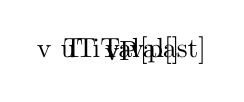
\begin{tikzpicture}
	 \tikzset{every tree node/.style={align=center,anchor=north}}
	\Tree [.TP [.DP  ] [.T'
	[.\node(T) {T {iT val[]}}; ] [.VoiceP [.DP\\Kofi ] [.Voice' [.voice ] 
	 [.\node (102){vP}; [.\node(v1){v uT val[past]};\\buy ] [.VP [.V ] [.DP\\food ] ]  ] ] ]
	 ]  
	]
%	\draw[dashed, -> ] (T.south) to [bend right=90] (v1.south);
%	\draw[dashed, -> ] (T.south) to [bend right=90] (v2.south);
\end{tikzpicture}
\caption{Agreement between tense and the verb  (before Agree)}
\end{figure}
\begin{figure}
\begin{tikzpicture}
	 \tikzset{every tree node/.style={align=center,anchor=north}}
	\Tree [.TP [.DP  ] [.T'
	[.\node(T) {T {iT val[past]}}; ] [.VoiceP [.DP\\Kofi ] [.Voice' [.voice ] 
	 [.\node (102){vP}; [.\node(v1){v uT val[past]};\\buy ] [.VP [.V ] [.DP\\food ] ]  ] ] ]
	 ]  
	] 
	\draw[dashed, ->] (T.south) to [out=270,in=240] ($(v1.south west)+(2.5em,0)$);
%	\draw[dashed, -> ] (T.south) to [bend right=90] (v2.south);
\end{tikzpicture}
\caption{Agreement between tense and the verb (after Agree)}
\end{figure}
 
Agree is thus a two-step process. For instance, the interpretable but unvalued tense feature on T,([iT val[]]), probes its c-command domain for the uninterpretable but valued tense feature on v, ([uT val[past]]). When it finds it, Agree is established, and T and V now shares the tense feature ([iT val[past]]) and ([uT val[past]]). If this Agree relation were not established, then the tense feature would not receive an interpretation. 

The Agree relation is, however, only defined for T Agreeing with a single head. For the T to Agree with multiple verbs, I propose a modification of  \citet{Hiraiwa2001}, which allows T to Agree with goals that are not in a c-commands relation. I refer to the modified Multiple Agree process as \textit{Parallel Agree} defined below.

\ea \label{ex25}
Parallel Agree with a single probe is a single simultaneous syntactic operation: Agree applies to all matched goals at the same derivational point. There is no c-command between the goals.
\z

\begin{figure}
	\begin{tikzpicture}
		\Tree [.a [.\node(A) {$\alpha$}; ] [.b [.c [.e ] [. \node(B) {$\beta$}; ] ] [.d [.f ] [.\node(Y) {$\gamma$}; ] ] ] ]
	\draw[->](A)..controls +(south west:2) and +(south west:2)..(B);
	\draw[->](A)..controls +(south west:2) and +(south west:2)..(Y);
	\end{tikzpicture}
\caption{Agree ($\alpha$, $\beta$, $\gamma$), where $\alpha$ is a probe and $\beta$ and  $\gamma$ are matching goals for $\alpha$ and they do not c-command each other.}
\end{figure}

With Parallel Agree, we can derive the Agree relation with the single T projection in SVCs with all the verbs in an SVC. This is illustrated below. 
 
\begin{figure}[p]
\caption{\label{ex35a}Parallel Agree with two past tenses (before Agree)}
\begin{tikzpicture}[scale=.75]
	 \tikzset{every tree node/.style={align=center,anchor=north}}
	\Tree [.TP [.DP  ] [.T'
	[.\node(T) {T {iT [ ]}}; ] [.VoiceP [.DP\\Kofi ] [.Voice' [.voice ] [.\node (V)  {vP};
	 [.\node (102){vP}; [.\node(v1){v uT val[past]};\\buy ] [.VP [.V ] [.DP\\food ] ]  ]  [.v' [.\node (V2)  {v}; $\emptyset$ ]  [.vP [.\node(v2){v uT val[past]};\\eat ] [.VP [.V ] [.DP ] ]  ]
	  ] ] ] ]
	 ]  
	]
	\draw[dashed, ->, overlay ] (T.south) to [bend right=90] ($(v1.south west)+(2.5em,0)$);
	\draw[dashed, ->, overlay ] (T.south) to [bend right=90] ($(v2.south west)+(2.5em,0)$);
\end{tikzpicture} 
\end{figure}

\begin{figure}[p]
\caption{\label{ex35b}Parallel Agree with two past tenses (after Agree)}
\begin{tikzpicture}[scale=.75]
	 \tikzset{every tree node/.style={align=center,anchor=north}}
	\Tree [.*TP [.DP  ] [.T'
	[.\node(T) {T {iT [\textsc{past} ]}}; ] [.VoiceP [.DP\\Kofi ] [.Voice' [.voice ] [.\node (V)  {vP};
	 [.\node (102){vP}; [.\node(v1){v uT val[past]};\\buy ] [.VP [.V ] [.DP\\food ] ]  ]  [.v' [.\node (V2)  {v}; $\emptyset$ ]  [.vP [.\node(v2){v uT val[past]};\\eat ] [.VP [.V ] [.DP ] ]  ]
	  ] ] ] ]
	 ]  
	]
	\draw[dashed, ->, overlay ] (T.south) to [bend right=90] ($(v1.south west)+(2.5em,0)$);
	\draw[dashed, ->, overlay ] (T.south) to [bend right=90] ($(v2.south west)+(2.5em,0)$);
\end{tikzpicture}
\end{figure}

In this derivation, T probes and matches with all the verbs then simultaneously Agree with them. The unvalued but interpretable T feature ([iT []]) on T applies to all the matched goals derivationally simultaneously, establishing Agree (iT[\textsc{pst}]...uT \emph{val}[\textsc{pst}]...uT \emph{val}[\textsc{pst}]).

Now we can explain the matching restriction in SVCs. Since T can only have one interpretable feature, we predict that for a sentence to be grammatical, all the verbs in the sentence must have the same tense feature. For instance, if the first verb is valued for past tense, and the second verb is valued for the present tense, T receives two different tense values to interpret, therefore, uninterpretable. 


\begin{figure}[p]
\caption{\label{ex36a}Parallel Agree with past tense and present tense  (before Agree)}
\begin{tikzpicture}[scale=.75]
	 \tikzset{every tree node/.style={align=center,anchor=north}}
	\Tree [.TP [.DP  ] [.T'
	[.\node(T) {T {iT [ ]}}; ] [.VoiceP [.DP\\Kofi ] [.Voice' [.voice ] [.\node (V)  {vP};
	 [.\node (102){vP}; [.\node(v1){v uT val[past]};\\buy ] [.VP [.V ] [.DP\\food ] ]  ]  [.v' [.\node (V2)  {v}; $\emptyset$ ]  [.vP [.\node(v2){v uT val[present]};\\eat ] [.VP [.V ] [.DP ] ]  ]
	  ] ] ] ]
	 ]  
	]
	\draw[dashed, ->, overlay ] (T.south) to [bend right=90] ($(v1.south west)+(2.5em,0)$);
	\draw[dashed, ->, overlay ] (T.south) to [bend right=90] ($(v2.south west)+(2.5em,0)$);
\end{tikzpicture} 
\end{figure}

\begin{figure}[p]
\caption{\label{ex36a2}Parallel Agree with past tense and present tense (after Agree)}
\begin{tikzpicture}[scale=.75]
	 \tikzset{every tree node/.style={align=center,anchor=north}}
	\Tree [.*TP [.DP  ] [.T'
	[.\node(T) {T {iT [\textsc{??} ]}}; ] [.VoiceP [.DP\\Kofi ] [.Voice' [.voice ] [.\node (V)  {vP};
	 [.\node (102){vP}; [.\node(v1){v uT val[past]};\\buy ] [.VP [.V ] [.DP\\food ] ]  ]  [.v' [.\node (V2)  {v}; $\emptyset$ ]  [.vP [.\node(v2){v uT val[past]};\\eat ] [.VP [.V ] [.DP ] ]  ]
	  ] ] ] ]
	 ]  
	]
	\draw[dashed, ->, overlay ] (T.south) to [bend right=90] ($(v1.south west)+(2.5em,0)$);
	\draw[dashed, ->, overlay ] (T.south) to [bend right=90] ($(v2.south west)+(2.5em,0)$);
\end{tikzpicture}
\end{figure}


\subsection{Aspect}\label{sec:owusu:4.2}
The central claim in this section is that \emph{à}- is the spell-out of an inner aspect head with content-less neutral features [−prog, −fut]. As we have already seen, \emph{à}- is only licensed in coordinate constructions, not in other multi-verb constructions. I argue that this is due to the asymmetric relationship between the external and internal complement in coordinate structures. The distribution of aspect is shown in (\ref{ex:04}) repeated here.

\begin{exe}
\exr{ex4}[]{V(Asp) \phantom {} {} {} V(à)\\
\gll Kofi \textit{re}-to boɔ \textit{à}-kɔ dan mu.\\
	Kofi \textsc{prog}-throw stone \textsc{cons}-go room  PostP\\
\glt `Kofi is throwing a stone for it to go into the room.'}
\exr{ex5}[*]{V(Asp)\phantom {} {} {}   V(Asp)\\
\gll  Kofi re-to boɔ re-kɔ-ɔ dan mu.\\
	  Kofi \textsc{prog}-throw  stone  \textsc{prog}-go room PostP\\} 
\exr{ex6}[*]{V(Asp)\phantom {} {} {}   V(Past)\\
\gll Kofi re-to boɔ kɔ-ɔ dan mu.\\
	 Kofi \textsc{prog}-throw  stone  go-\textsc{pst} room PostP\\}
\end{exe}

Cross-linguistically, aspect is thought to be below T, (see \citet{Rizzi2004} \citet{Rizzi2013Notes}, a.o, \citet{Cinque2002, Cinque2006}, \citet{RizziCinque2016} \citet{CinqueRizzi2010} a.o). Following \citet{Kandybowicz2010, Kandybowicz2015}, I argue that aspect in Akan is merged lower, i.e., within the vP.  However, as a quantifier of events \citep{Hacquard2006}, aspect is only interpretable above vP; therefore, aspect is not interpreted where it is base-generated in Akan. To solve this apparent mismatch, I argue that there is another aspect projection above vP, where aspect is interpreted. I refer to this projection as outer aspect. Inner aspect is the morphological projection of aspect.\footnote{The idea of two aspect projections in the syntax is a not new, inner aspect is used to refer to lexical aspect/situational aspect while outer aspect to grammatical/viewpoint aspect (see \citealt{Travis2010, Travis1991, Smith1991, MacDonald2006}). In Tagalog and Navajo, Inner aspect also encodes grammatical aspect \citep{Travis2010}.} Descriptively, Outer aspect and inner aspect are required to be compatible or match. Matching is checked through \textit{Selection/Sel(ect)-Merge}. The proposal is that Outer aspect \textit{selects} for an inner aspect with compatible features. Since Outer aspect and Inner aspect are not sisters, 
I assume that aspect features percolate to VoiceP, the sister of Outer aspect, where compatibility is checked. \citegen{Webelhuth1992} percolation principles govern the feature percolation. \nocite{Webelhuth1992}
\eanoraggedright \label{ex16}
\ea If the head of XP is marked for the feature F, then F percolates to the XP. (same as projection of head features to maximal projections in the Minimalist framework)
\ex If the head of XP is not marked for F and spec of XP is marked for F, then F percolates from the specifier to the XP. (This could be done via the head, using spec-head agreement.)

\ex If neither the head of XP or spec XP is specified for a value of F(+\,or\,−) and complement is specified, then complement can percolate features to XP. 
\z
\z
These principles determine where features can percolate from.
 
Inner aspect is associated with three morphosyntactic feature bundles; [+prog, −fut] ({progressive}) , [+fut, −prog] ({future}) and [−prog, −fut] (\emph{à}).  \emph{à} has no semantic input. The interpretation of aspect is the union of outer aspect and inner aspect, but since Outer aspect has no value, Inner aspect determines the value of the construction. Through percolation, inner aspect features get to VoiceP where Outer aspect can check them for selection.  I argue that since \emph{à} has no semantic input, it is infelicitous in any position where it has to contribute to interpretation. This is what happens in the simple clause as in (\ref{ex8}). In a simple clause, the feature bundle of \emph{à'}  percolate to VocieP where it is accessible to Outer aspect, but there is no interpretable aspect features. We can extend the same argument to all contexts where consecutive \emph{à}- is not felicitous. For instance, as the verb in an SVC, the features of \emph{à}- has to percolate to Outer aspect for interpretation. The analysis here borrows the idea from  \citet{Zhang2009} that the external conjuncts are privileged, i.e., it is only the features of the external conjunct that are relevant for feature selection. 

For instance, a verb that does not select for a CP complement can take a conjoined DP and CP as its complement as long as they are in that order. In (\ref{ex39}), though the preposition \emph{ on} selects a DP, it can take a conjoined DP and CP, only if the DP is in the external conjunct.
\ea\label{ex39}
\ea You can depend on \textit{my assistant} and \textit{that he will be on time}. (DP \& CP)

\ex You can depend on \textit{that he will be on time}.

\z 
\z  In the same way, \emph{à}-  is only licensed in the internal conjunct of a coordinate clause. The \emph{à}-[+prog, −fut] in an internal conjunct position does not percolate to VoiceP and is not selected by Outer aspect for interpretation. The only features that are accessible to the outer aspect are the Inner aspect features in the external conjunct. The tree in \figref{fig:ex40} is a representation of example (\ref{ex4}) above.\footnote{A reviewer notes that the feature percolation proposed leads us to expect arbitrarily long-distance morphological dependencies. This is indeed a problem for feature percolation. For now I assume that features can percolate until they met an operator that check those features.}  

\begin{figure}
\caption{Percolation of aspect features\label{fig:ex40}}
\begin{tikzpicture}[scale=.75]
	 \tikzset{every tree node/.style={align=center,anchor=north}}
	\Tree [.TP [.DP\\Kofi ] [.T'
	[.T ] [.NegP [.Neg ] [.OAspP [.OAsp\\re ] [.\node(110){VoiceP+prog,−fut}; [.DP ] [.\node (105){Voice'+prog,−fut}; [.Voice ] [.\node (V)  {vP+prog,−fut};
	 [.\node (102){vP+prog,−fut}; [.v\\to ] [.\node (101){IAspP+prog,−fut}; [.\node (100){IAsp\\{[+prog,−fut]}}; ] [.VP [.V ] [.DP\\boɔ ] ] ] ]  [.v' [.\node (V2)  {v}; $\emptyset$ ]  [.\node (vpp) {vP{−prog,−fut}}; [.v ] [.\node (ok){IAspP{−prog,−fut}\\}; [.\node (okk){IAsp\\{[−prog,−fut]}}; ] [.VP [.V\\kɔ ] [.PP [.DP [.NP\\dan ] [.D\\no ] ] [.P\\mu ] ] ] ] ]
	  ] ] ]
	 ] ] ]
	] ]
	\draw[dashed,-> ] (100.west) to [bend left=60] (101.west); % ok
	%\draw[->](100)..controls +(south west:2) and +(west:2)..(101)node[near end, left] {\scriptsize feature percolation};
	\draw[dashed,-> ] ($(101.north east)+(-1em,0)$) to [bend right=60] (102.east); % ok
	\draw[dashed,-> ] ($(102.north west)+(1.5em,0)$) to [bend left=60] (V.west); % ok
	\draw[dashed,-> ] ($(V.north east)+(-1.5em,0)$) to [bend right=60] (105.east); % ok
	\draw[dashed,-> ] ($(105.north east)+(-1.5em,0)$) to [bend right=60] (110.east); % ok
    \draw[dashed,-> ] (okk.west) to [bend left=60] ($(ok.west)+(0,0.5em)$);
    \draw[dashed,-> ] ($(ok.north east)+(-1.5em,0)$) to [bend right=60] (vpp.east);
\end{tikzpicture}  
\end{figure}

This same logic can be used to account for the ungrammaticality of \emph{à} in both the *{V(à)} {V(à)} and *{V(à)} {V(Asp)} sequence. But nothing I have said so far rules out having two overt aspects with interpretation, i.e.,*{V(Asp)} {V(Asp)}, though empirically it is ungrammatical. I derived the ungrammaticality of these sequence from an economy of interpretation principle modeled after \citet{Boskovic1997Book} minimal structure principle.

\ea
Economy of interpretation\\
Provided that lexical requirements of relevant elements are satisfied, if two representations have the same gross syntactic structure and have the same interpretation, then the version that has fewer \emph{+features} is chosen as the morphosyntactic representation serving that function.
\ex \label{ex41}
\ea[*]{re  (+prog, −fut) + re  (+prog, −fut)}
\ex[*]{re (+prog, −fut) + bɛ (−prog, +fut)}
\ex[]{\label{ex41c}re (+prog, −fut) + \emph{à}- (−prog, −fut)}
\z
\z
Based on the privileged position of external conjuncts of coordinate structures and the fact that the feature percolation principle requires that features percolate from the specifier, all the cases in (\ref{ex41}) end up with the same aspect interpretation. As such, semantically they serve the same function. Therefore, the simplest version,i.e., (\ref{ex41c}), with the least number of \emph{+features} is chosen. 


\section{Conclusion}\label{sec:owusu:5}
I have argued that tense and aspect have different distributions in these clauses because they are governed by distinct mechanisms, tense by Agree and aspect by Selection. The -\emph{à} morpheme that appears on the non-initial verbs in these clauses is the phonological realizations of the morphosyntactic feature bundles [−prog,−fut] of inner aspect. It is only licensed in a position where its aspectual features do not percolate to a VoiceP. Tense morphology depicts T-v Agree. There are multiple instances of tense because a single T head parallel-Agrees with all the verbs. Single T-head Agree results in the matching restriction. This difference in the mechanism used for the valuation of features is not arbitrary; it is governed by the position of the syntactic objects involved. There is one T merged in these constructions but multiple verbs with tense features that need to be checked, the single T thus enter into an Agree relation with all of them.  Aspect, on the other hand,  is merged multiple times 



%The proposed Parallel Agree configuration --- in which two goals are not in an asymmetric c-command relationship --- poses problems for certain definitions of Shortest, a widely assumed requirement on Agree (as well as movement chains). This should minimally be noted.
%Feature percolation of the sort proposed for Akan aspect seems, as is, to pose a potential problem: it leads us to expect arbitrarily long-distance morphological dependencies to be expressed. This problem should be noted, or something should be said to limit the domains in which feature percolation might take place.
\section*{Abbreviations}
\begin{multicols}{3}
\begin{tabbing}
PostP\hspace{.5ex} \= Postposition\kill
\textsc{cons}  \> Consecutive \\ \> Morpheme  \\
Cord  \> Coordinator \\
\textsc{fut}  \> Fut \\
\textsc{perf}  \> Perfect \\
PostP \> Postposition  \\
\textsc{pres}  \> Present  \\
\textsc{prog}  \> Progressive \\
\textsc{pst}  \> Past
\end{tabbing}
\end{multicols}

\section*{Acknowledgments}
The chair of my second qualifying paper, Professor Mark Baker and my committee members, Ken Safir and Viviane Deprez help shaped most of the ideas in this paper. I would like to thank the Rutgers syntax reading group (STAR), your comments and insights helped improve this paper. I am also grateful to the participants of ACAL\,49, your questions and comments were beneficial. I have benefited from the comments and insights of two anonymous reviewers.

{\sloppy\printbibliography[heading=subbibliography,notkeyword=this]}
\end{document}
